\documentclass{article}
\usepackage{amsmath}
\usepackage{amssymb}
\usepackage{graphicx}
\usepackage{hyperref}
\usepackage[version=4]{mhchem}


\begin{document}
\section*{Problem}
In a circle with center \(O\) chord \(A B=\) chord \(A C\). Chord \(A D\) cuts \(B C\) in \(E\). If \(A C=12\) and \(A E=8\), then \(A D\) equals:\\
(A) 27\\
(B) 24\\
(C) 21\\
(D) 20\\
(E) 18\\
\centering
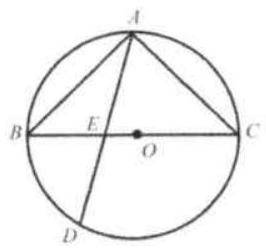
\includegraphics[width=\textwidth]{images/170.jpg}

\section*{Solution}
(E).\\
Since \(A B=A C, \angle A C B=\angle A B C=\alpha\).\\
Connect \(B D\).\\
\(\angle A D B=\angle A C B=\alpha(\) they face the same \(\operatorname{arc} A B)\).\\
Then triangles \(A B E\) and \(A D B\) are similar to each other, so the following equality holds true: \(\frac{A B}{A D}=\frac{A E}{A B}\)\\
\(\Rightarrow \quad \frac{12}{A D}=\frac{8}{12}\)\\
\(\Rightarrow \quad A D=18\)\\
\centering

\includegraphics[width=\textwidth]{images/174.jpg}

Method 2:\\
Connect \(C D\).\\
Let \(\angle E A C=\angle B A C=\alpha\).\\
\(\angle A C B=\angle A D C=\beta\) (they face the arcs of the same length: \(\operatorname{arcs} A C, A B)\).

Then triangles \(A E C\) and \(A C D\) are similar to each other, so the following equality holds true: \(\frac{A C}{A E}=\frac{A D}{A C}\)\\
\(\Rightarrow \quad \frac{12}{8}=\frac{A D}{12}\)\\
\(\Rightarrow \quad A D=18\)\\
\centering
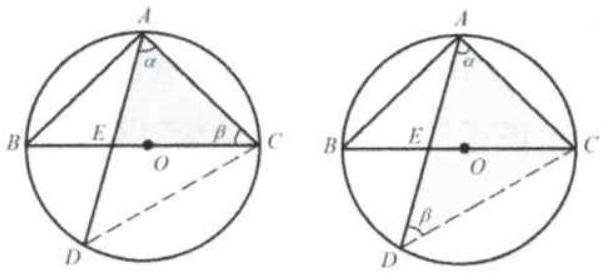
\includegraphics[width=\textwidth]{images/174(1).jpg}


3. When two circles are tangent or intersecting, draw the common tangent line, the common chords, or connect the centers.
3.1. Circle \(O_{1}\) and \(O_{2}\) are tangent. Draw the common tangent line \(A B\). Connect \(O_{1} A\) and \(O_{2} B\). Connect \(O_{1} O_{2}\). Draw \(O_{1} C / / A B\).\\
\centering
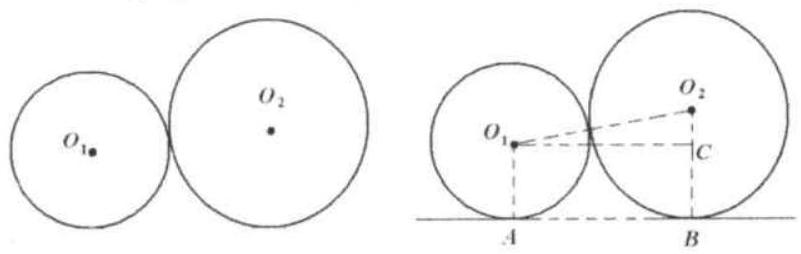
\includegraphics[width=\textwidth]{images/175(1).jpg}

We have\\
\(A B=O_{1} C\).\\
\(A B \perp O_{1} C\).\\
\(A B \perp O_{2} B\).\\
\(O_{1} O_{2}=r_{1}+r_{2}\).\\
\(O_{2} C=r_{2}-r_{1}\).\\
\(\triangle O_{1} \mathrm{CO}_{2}\) is a right triangle.\\
\(O_{1} C=\sqrt{\left(r_{2}+r_{1}\right)^{2}-\left(r_{2}-r_{1}\right)^{2}}\)\\
\(r_{1}\) and \(r_{2}\) are the radius of circle \(O_{1}\) and \(O_{2}\), respectively.\\
3.2. Circle \(O_{1}\) and \(O_{2}\) are intersecting at \(E\) and \(F\). Draw the common tangent lines \(A B, C D\), respectively. Connect \(O_{2} C, E F\), and \(O_{1} O_{2}\).\\
\(O_{1} O_{2}\) is the perpendicular bisector of \(E F . O_{2} C \perp D C\).\\
\centering

\includegraphics[width=\textwidth]{images/175.jpg}

Theorem 6.9. Any point on the perpendicular bisector of a line segment is equidistant from the endpoints of the line segment. Two points equidistant from the endpoints of a line segment determine the perpendicular bisector of the line segment.

\end{document}
